\chapter{Introduction to Machine Learning Toolkits}
\label{chp:Toolkits}
We have used two state-of-the-art machine learning toolkits in our project, to help us achieve our goals. These tools are:-
\begin{itemize}
    \item Intel OpenVINO computer vision toolkit
    \item Tensor Virtual Machine (TVM)
\end{itemize}
Both these tools have the same high level goal, that being the deployment of pre-trained CNN models on different hardware platforms such as CPU, GPU, FPGA etc. thereby making the high level deep learning frameworks such as Tensorflow, Caffe etc. independent of the underlying hardware. However, none of these tools alone can achieve our goals, making it necessary to use a combination of both, using certain components and features in each toolkit. Both Intel OpenVINO and TVM are described in detail in the next sections.  

\section{Intel OpenVINO}


Intel OpenVINO is an open source toolkit from Intel that allows the deployment of pre-trained deep neural networks on different hardware platforms such as CPU, GPU, FPGA, etc. The toolkit is available for installation for the Windows operating system as well as selected Linux distributions. All of the tool's libraries and plugins except the FPGA plugin are a part of the open source GitHub repository.
The functionality of OpenVINO is divided among its components, Model Optimizer and Inference Engine. This is shown in Figure \ref{fig:OpenVINO_workflow} and explained below. 
\begin{figure}[!hbpt]
    \centering
    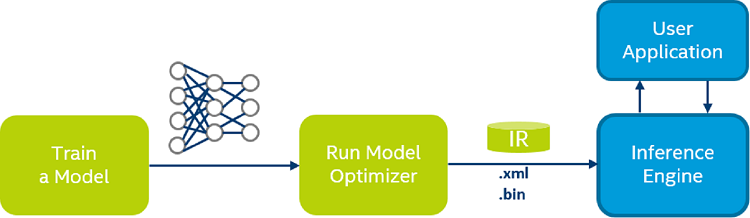
\includegraphics[width=0.65\textwidth]{img/openVINO_workflow.png}
    \caption{Intel OpenVINO workflow \citep[][]{openvino_fig}}
    \label{fig:OpenVINO_workflow}
\end{figure} 

\subsection{Model Optimizer}
The Model Optimizer is a python based tool which takes as input a pre-trained model. It supports many popular deep learning frameworks such as TensorFlow, Caffe, PyTorch, MXnet, etc. This model is then converted to a common intermediate format (IR), thereby making the inference engine independent of the training framework. The IR contains a .xml file which represents the computational graph of the CNN and a .bin file containing the weights. The graph is optimized by fusing different layers of the original topology wherever possible. Typically the batch normalization layers are fused with their preceding convolution layer and the convolution filter weights are accordingly adjusted. The toolkit comes with a model downloader which can download various openly available pre-trained models for different frameworks.
 

 \subsection{Inference Engine}
 The Inference Engine is responsible for the execution of the model on the selected hardware. For this purpose, it provides a C++ API which can be integrated into an application. The main task performed by the inference engine is to read the intermediate representation of the model, select the hardware for deployments such as CPU or FPGA and call the appropriate plugin which defines all necessary data structures and functions required to perform inference and return the output along with performance statistics. 
 The toolkit comes with pre-compiled bitstreams for a few supported FPGA boards. These bitstreams implement various popular network topologies such as GoogLeNet, ResNet, etc. as well as generic layers which are used to program the FPGAs as per the requirement of the given model topology.
 
 These bitstreams however, do not support the Intel Stratix 10 FPGA boards available in the Noctua infrastructure. In addition to this, the FPGA plugin of the inference engine is not open source, making it infeasible to use OpenVINO as a stand alone tool to achieve our project goals without customizing its components at the source code level.
 
 \subsection{OpenVINO source code}
 The Intel OpenVINO toolkit is open source and the code is available as a Github repository known as Deep Learning Deployment Toolkit (DLDT). The repository contains source code for both the Model Optimizer as well as the Inference Engine except for the FPGA plugin. As a result, we have written our own FPGA plugin for OpenVINO to support the Noctua infrastructure and enable scaling of CNNs over multiple FPGAs. 
 
 \subsection{FPGA plugin}
 The main purpose of the FPGA plugin is to flash the bitstreams (.aocx files) for the CNN models on the FPGAs and to launch the kernels according to the CNN topology. It also supports scaling on multiple FPGAs which has been achieved through the use of MPI (Message Passing Interface) and the serial I/O channels present between FPGA nodes in the Noctua infrastructure. 
 
 The plugin interacts with the Inference Engine C++ API which helps in parsing the intermediate representation obtained from the model optimizer for a given CNN model. We have reused the classes and data structures in this API as much as possible, specifically for parsing the .xml file in the IR containing the topology for the given CNN model, parsing the weights in the binary (.bin) file as well as parsing the input images. We have stored all the parsed information from the IR in a C++ struct for each layers. The definition of the struct is shown in the code snippet Code \ref{code:struct}.
 \begin{code}[!htb]
 \begin{minted}{c++}
 /**
 * Data structure to store information of each layer
 */
struct layersDetails
{
	//Layer ID
	int layerID;
	// Layer Name
	std::string layerName;
	//Type of Layer
	std::string layerType;
	//Pointer to the Layer Bias vector
	float *layerBias;
	//Pointer to the Layer Weights vector
	float *layerWeights;
	//Total number of biases
	int num_biases;
	//Total number of weights
	int num_weights;

	//Hashmap for parameters ( kernel, padding,dilation,precision) with its values.
	std::map<std::string, std::string> params;
	//Vector of parent layers
	std::vector<std::string> inputLayerNames;
	//Vector of child layers
	std::vector<std::string> outputLayerNames;
	//Vector of pointers to the Layers Details Structure of Children nodes
	std::vector<struct layersDetails *> children;
	//Vector of pointers to the Layers Details Structure of parent nodes
	std::vector<struct layersDetails *> parents;

	// Buffer index of the output
	int layerOutBufferIndex = 0;
	// vector of buffer index
	std::vector<int> parentOutBufferIndex;
	// Output dimension
	int outH = 0, outW = 0, outDepth = 0;
	//Flag to check if layer is executed.
	int visited = 0;
};

    
\end{minted}
\caption{Struct to store parsed IR information for each layer in CNN}
\label{code:struct}
\end{code}
 
 In addition to this pre-existing source code, we have written our own tree data structure in the plugin, to represent the CNN topology in a suitable pointer structure that adequately models the input output relationships between CNN layers, thus allowing us to launch their corresponding OpenCL kernels in an orderly fashion. 
 
 The plugin also supports scaling over multiple FPGAs, through the use of MPI and dedicated serial I/O connections between FPGA boards that are present in the Noctua infrastructure. The infrastructure consists of 16 FPGA nodes, each hosting 2 Intel Stratix 10 FPGA boards. Our plugin has multiple instances running as MPI processes, one per node. Each plugin instance is thus responsible for the execution of partial CNN topology on 2 FPGAs. We divide the CNN model at the OpenCL level into multiple .cl files which are then synthesized to generate their corresponding bitstreams. These bitstreams are then named in a suitable fashion so as to create a mapping between them and the specific plugin instance running on a FPGA node which is identified by its MPI rank. To map the names of the CNN layers (OpenCL kernels) to the .aocx file that contains them, we use Intel OpenCL SDK binutils to generate a .xml file corresponding to each .aocx bitstream. The plugin instance would thus flash appropriate .aocx files according to its MPI rank and then launch appropriate kernels that are contained in those .aocx files, after parsing the corresponding xmls. 
 
 The sequence diagram in the Figure \ref{fig:plugin_uml} shows the operations during the execution of the plugin.
 \begin{figure}[!hbpt]
    \centering
    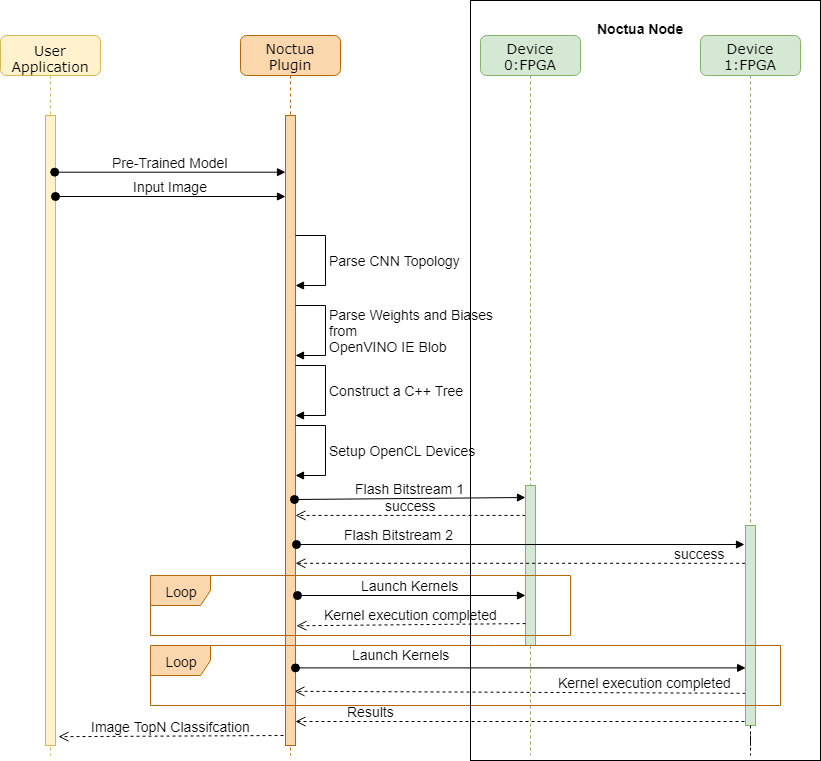
\includegraphics[width=\textwidth]{img/Plugin_UML_1.png}
    \caption{Sequence diagram of the Inference Engine at one node}
    \label{fig:plugin_uml}
\end{figure} 

 \begin{itemize}
     \item The user application sends the CNN model IR and the input image to the plugin.
     \item The FPGA plugin parses the IR, both the xml and bin files to retrieve the layer information and the weights which are then used to construct a tree data structure.
     \item The plugin instance then flashes the appropriate bitstreams on the FPGA boards and parses their corresponding xml files to get a mapping between the aocx files and the kernel names.
     \item The kernels are then launched by a level wise traversal of the tree structure representing the CNN model.
     \item One instance of the plugin is executed parallelly at every node.
     \item The plugin instance at the last node collects results and returns them to the user application which displays the top N labels and their softmax scores (confidence) to the user.
 \end{itemize}
 
 \subsection{Advantages}
  
 \begin{itemize}
 \item Supports optimization of models and quantization of weights.
 \item A CNN model can be deployed on hardware with minimal programming effort and independent of the training framework.
 \item For FPGAs, the use of pre-compiled bitstreams eliminate the time needed for synthesis of kernel codes.
 \end{itemize}
 
 \subsection{Disadvantages}
 \begin{itemize}
 \item The main disadvantage is the compatibility of FPGA boards. Development and synthesis of kernel codes along with a plugin for FPGAs may be required to make OpenVINO work with unsupported boards. 
 \item Scaling to multiple FPGAs, which is one of the goals of this project is non-trivial as it would require the development of overlays for external I/O channels. 
 \end{itemize}
\section{TVM}
There is an increasing demand for implementing machine learning on a wide variety of hardware devices. Many frameworks rely on hardware vendor-specific libraries and optimize for very specific GPUs. Deploying a machine learning model on a new platform needs a lot of trial and error manual efforts. Mapping Deep Learning (DL) models to specific hardware are complicated by diversity in hardware functionality. Various hardware such as CPU, GPU, FPGAs, and ASICs have a quite different on-chip memory architecture and compute primitive. Tensor Virtual Machine (TVM) is an open-source compiler and code generator that uses graph-level and operator-level optimizations to build and deploy deep learning models on diverse accelerators (e,g, FPGAs, ASICs).

DL frameworks such as Tensorflow, Caffe, and PyTorch rely on a computational graph intermediate representation to implement optimizations such as auto differentiation and dynamic memory management. TVM includes a computational graph rewriter, tensor expression language and new features for GPU accelerators. The TVM compilation stack is shown in Figure \ref{fig:tvm_fig}.

\begin{figure}[h!]
    \centering
    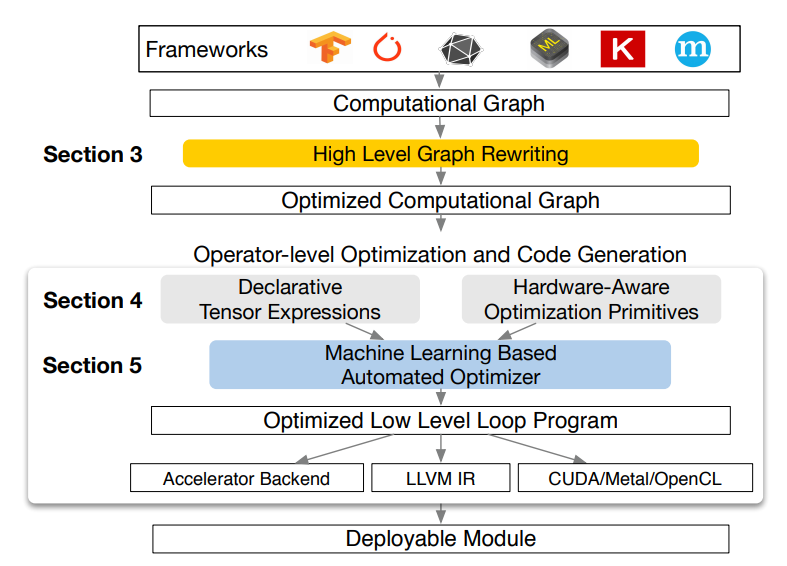
\includegraphics[scale=0.50]{tvm_overview.png}
    \caption{System overview of TVM \cite{tvm_fig}}
    \label{fig:tvm_fig}
\end{figure}

TVM takes a deep learning model in the form of a frozen \textit{protobuf} file and transforms it into a computational graph representation. TVM performs high-level optimizations such as dataflow rewriting to generate an optimized graph. In operator-level optimizations, various operators are fused together efficiently and are used for code generation. All the operators are specified in a declarative tensor expression language and TVM checks for possible hardware operators optimizations based on the selected target hardware accelerator. The cost model is used to find the optimized operators and the generated code is compiled together into a deployable module.

 \begin{code}[!htb]
 \begin{minted}{Python}
target = 'aocl_sw_emu'
target_host = 'llvm'
layout = 'NCHW'
ctx = tvm.cpu(0)

img_path = download_testdata(image_url, img_name, module='data')

model_path='resnet_frozen.pb'

with tf.gfile.FastGFile(model_path, 'rb') as f:
    graph_def = tf.GraphDef()
    graph_def.ParseFromString(f.read())
    graph = tf.import_graph_def(graph_def, name='')
    graph_def = tf_testing.ProcessGraphDefParam(graph_def)
    # Add shapes to the graph.
    with tf.Session() as sess:
        graph_def = tf_testing.AddShapesToGraphDef(sess,
        'resnet_v2_50/predictions/Reshape_1')   

from PIL import Image
image = Image.open(img_path).resize((224, 224))

shape_dict = {'DecodeJpeg/contents': x.shape}
dtype_dict = {'DecodeJpeg/contents': 'uint8'}

sym, params = nnvm.frontend.from_tensorflow(graph_def, layout=layout,
shape=shape_dict)


with nnvm.compiler.build_config(opt_level=3):
    graph, lib, params = nnvm.compiler.build(sym,  target=target,
    target_host=target_host,  params=params)


\end{minted}
\caption{TVM Python API code for ResNet-50}
\label{code:TVMAPI}
\end{code}


In Code \ref{code:TVMAPI}, we use TVM API to get OpenCL generated code for ResNet-50 model.
After compilation we have three components variables: the optimized computational graph, generated operators for the target library and final parameters after compilation. The computational graph also provides us with intermediate representation and mapping of the code generated with its respective inputs.

\pagebreak

Computational graphs provide an overall view of the operators but lack specifying information about how to implement those operators. TVM performs various graph level optimizations such as:
\begin{itemize}
 \item Operator fusion – Combiles multiple operations into a single kernel and thus helps us in reducing execution time.
 \item Constant folding – Certain graph values can be pre-computed statistically.constant folding helps us to compute those values.
 \item Static memory planning pass – Pre-allocates memory to store intermediate tensor.
 \item Data layout transformation - Helps us to convert the computational graph into internal layouts specific to the target hardware.

 \end{itemize}
 
 Following are the important components of TVM.
 
 \subsection{Compilers}
 TVM provides us two types of compilers.
 
 
 \subsubsection{NNVM}
 
 NNVM compiler applies graph level and tensor level optimizations to generate target hardware code. NNVM provides us with pre-defined core tensor operator primitives. \textit{tennvm.top} (Tensor operator property registry) provides information about which operators can be scheduled together and is the basic building block for the optimization.
 
 NNVM has four levels of operators :
 
 \begin{itemize}
    \item Level 1: Basic Operators - This level includes vary basic operators such as \textit{dense}, \textit{Relu}, \textit{sigmoid}, \textit{exp}, etc.
    \item Level 2: Convolutions - The operators related to convolution become part of this level. Eg. \textit{con2d}, \textit{max\_pool2d}, \textit{avg$textunderscore$pool2d}, etc.
    \item Level 3: Additional Tensor Operators - Operations that provide the additive feature to the original tensors are group together at this level. Eg- \textit{reshape}, \textit{floor}, \textit{round}, etc.
    \item Level 4: Broadcast and reductions - Operators such as \textit{sum}, \textit{mean}, \textit{max},  \textit{min} are part of the reduction level.
 \end{itemize}
 
 NNVM has following functionality:
 
 \begin{itemize}
    \item \textit{nnvm.frontend} take in the model provided by DL frameworks and generates NNVM compatible symbols and parameters (NDArray) which are used by NNVM.
    \item  \textit{nnvm.compiler} has  \textit{nnvm.build} and  \textit{nnvm.build\_config} functions.
    \item In \textit{build\_config} function we provide optimization level based on which graph and tensor optimizations are carried out.
    \item \textit{nnvm.build} function is used to make C API call for code generation with optimized computational graph (graph), target hardware (targer\_host), input parameters (param) and layout provided. 

 \end{itemize}
 
 TVM provides us with the following types of optimizations.
 
 \begin{itemize}
     \item Pass 0 \textit{SimplifyInference} -
It is usually carried out on batch normalization tensor operators.
 \item Pass 1 \textit{OpFusion} -
In \textit{OpFusion}, basic operators are fused together with the convolution layer along with the precomputation of tensor operators.
\item Pass  2 \textit{PrecomputePrune} -
In this level of optimization, tensor operators can be pre-computed statistically during compilation time and replaced with a variable value thus reducing the operations required for the kernel.
\item Pass  3 \textit{FoldScaleAxis} -
In \textit{FoldScaleAxis} algorithm, the idea is to transform expression to a tuple of value, axes, and scale, where the following holds,
\begin{code}[!htb]
 \begin{minted}{Python}

 result = value
 for i, k in enumerate(axes):
    k-th dimension of result *= i-th dimension of scale
 \end{minted}
\end{code}
This is propagated along the signal and scale is folded if necessary. To ensure all scales are accessed, backward “preparation phase” propagation checks if potential axes scale back to its input.
We have used this optimization level during our kernel generation
 \end{itemize}
 
  \subsubsection{Relay}
Relay is known as NNVM {$V_2$}. It is a high-level functional IR for TVM.  Relay has 8 levels of definitions and is finely grained with extended support of \textit{Image operators}, \textit{Algorithm operators}, \textit{Temporary operators}, and \textit{dialect operators}. It distinguished between local and global variables been used.

\begin{itemize}
    \item Relay uses similar levels of optimizations as NNVM.
    \item \textit{relay.backend}  is the python interface for relay interpreters.
    \item \textit{relay.frontend},  \textit{relay.build}  and \textit{relay.build\_config}  has similar functionality to its predecessor.
\end{itemize}

 \subsection{TOPI}
 TVM Operator Inventory (TOPI) is the operator collection library for TVM. It contains a list of predefined operators that are used to compute operator declaration while generating computational graph. List of operators supported by TOPI are \textit{identity}, \textit{negative}, \textit{floor}, \textit{ceil}, \textit{abs}, etc.
 \begin{itemize}
\item \textit{topi.identity(x)} Take identity of input x
\item \textit{topi.negative(x)} Take negative of input x
\item \textit{topi.abs(x)}  Take absolute value of the input of x, element-wise.
 \end{itemize}
 
 \subsection{Codegen}
 Code generation is implemented in \path{src/codegen} subdirectory of TVM. When we execute \textit{nnvm.compiler.build} function, a C++ API call is made to codegen library which is implemented in C++. API calls are first registered python \path{/tvm/api.py} from NNVM compiler which in turn calls \path{src/api/api_lang.cc} its C++ counterpart.
 
  \begin{code}[!htb]
 \begin{minted}{c++}
 TVM_REGISTER_API("_Placeholder")
.set_body([](TVMArgs args,  TVMRetValue* ret) {
    *ret = placeholder(args[0],
                       args[1],
                       args[2]);
  });
 \end{minted}
\caption{TVM Register API for Placeholder Operation}
\label{code:TVMRegisterAPI}
\end{code}
TVM uses \textit{TVM\_REGISTER\_*} function to expose C++ functions to Python. In Code \ref{code:TVMRegisterAPI} a register call made to placeholder operation for Resnet-50 kernel generation.
 
 \begin{code}[!htb]
 \begin{minted}{c++}
 runtime::Module Build(const Array<LoweredFunc>& funcs,
                      const std::string& target) {
  std::string mode = target;
  size_t pos = mode.find(' ');
  if (pos != std::string::npos) {
    mode = mode.substr(0, pos);
  }
  std::string build_f_name = "codegen.build_" + mode;
  // the build function.
  const PackedFunc* bf = runtime::Registry::Get(build_f_name);
  CHECK(bf != nullptr)
      << "Target " << target << " is not enabled";
  runtime::Module m = (*bf)(funcs, target);
  return m;
}
\end{minted}
\caption{TVM codegen Build() function}
\label{code:TVMCodegen}
\end{code}

 The \textit{Build()} function looks up the code generator for the given target in the \textit{PackedFunc} registry. Code \ref{code:TVMCodegen} shows build function our target library is AOCL. A \textit{Packedfunc} implements interoperability between C++ and Python for TVM. Due to interoperability, a Python function can be easily called from C++ codebase making it a bidirectional connection. A \textit{PackedFunc} helps use make API calls type-erased, which removes the restriction for the function to be bound to specific input and return from C++ codebase. The \textit{PackedFunc} wraps the input argument to \textit{TVMArgs} and results are returned via \textit{TVMRetValue}. In Code \ref{code:TVMCodegenRegisterAPI} \textit{set\_body} is the \textit{PackedFunc} for the API. Since target hardware for our project has been set to aocl, \textit{Build()} function registers \textit{codegen.build\_aocl}.
 
  \begin{code}[!htb]
 \begin{minted}{c++}
  TVM_REGISTER_API("codegen.build_aocl")
.set_body([](TVMArgs args, TVMRetValue* rv) {
    *rv = BuildAOCL(args[0], args[1], false);
  });
\end{minted}
\caption{TVM codegen register API}
\label{code:TVMCodegenRegisterAPI}
\end{code}

\textit{BuildAOCL()} function generates OpenCL kernels from the lowered IR using \textit{CodeGenAOCL} class. In lowered IR a high-level nest loop structure is transformed into low-level target hardware IR.

 \begin{code}[!htb]
 \begin{minted}{c++}
runtime::Module BuildAOCL(Array<LoweredFunc> funcs, std::string target_str,
                          bool emulation) {
  // Get code.
  using tvm::runtime::Registry;
  bool output_ssa = false;
  CodeGenOpenCL cg;
  cg.Init(output_ssa);
  for (LoweredFunc f : funcs) {
    cg.AddFunction(f);
  }
  std::string code = cg.Finish();
  if (const auto* f = Registry::Get("tvm_callback_opencl_postproc")) {
    code = (*f)(code).operator std::string();
  }

  // Write a .cl file.
  runtime::SaveBinaryToFile("aocl.cl", code.c_str());
\end{minted}
\caption{BuildAOCL() kernel generation}
\label{code:TVMCodegenBildAOCL}
\end{code}

\textit{BuildAOCL()} function parses through \textit{loweredFunc} and stores the code in \textit{aocl.cl} file. Fig 6.7 shows functionality of \textit{BuildAOCL()}

 \subsection{VTA}
 Versatile Tensor Accelerator (VTA) is a customizable deep learning accelerator with a TVM-based compiler stack. It is used for fast and efficient dense linear algebra and implements RISC-like processors for performing tensor operations.  VTA has four modules that communicate with each other using FIFO queues and local memory blocks (SRAM).  Module communication helps in establishing task-level pipeline parallelism.
\begin{itemize}
\item \textit{Fetch Module} – Loading and decoding instruction streams from global memory blocks (DRAM) and routing them to command queues.
\item \textit{Load Module} - Loading input and weight tensors from DRAM into data-specialized on-chip memories.
\item \textit{Compute Module} – Performs dense linear algebra. Loads data from DRAM and micro-operation kernels into register file and micro-op cache respectively.
\item \textit{Store Module} – Stores results from \textit{compute module} into DRAM.
 \end{itemize}
 
 \begin{figure}[h!]
    \centering
    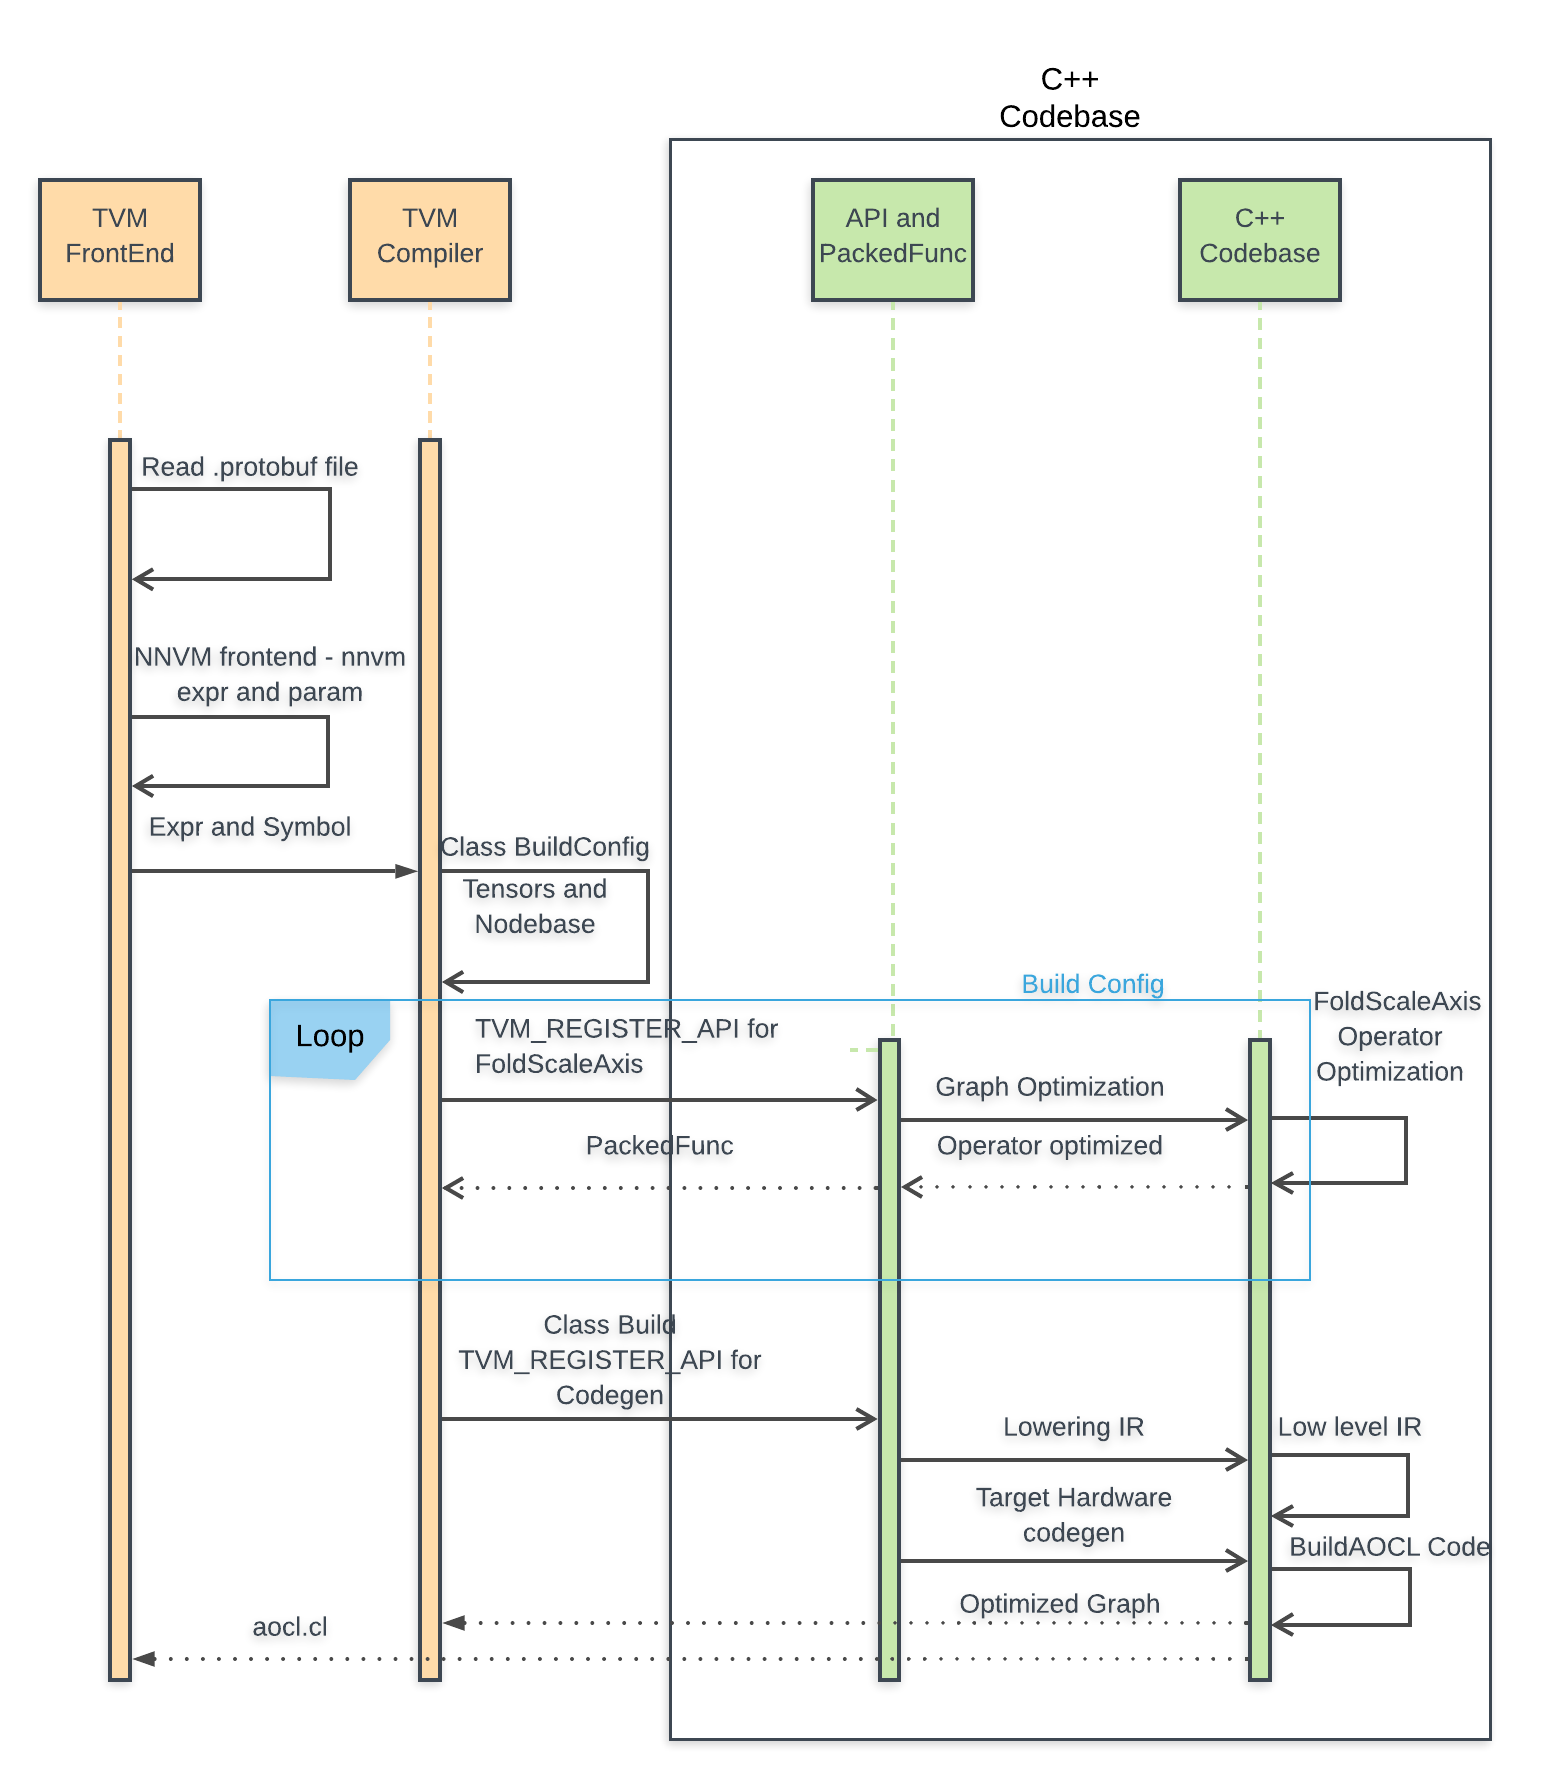
\includegraphics[scale=0.30]{tvm_workflow.png}
    \caption{Sequence diagram of Kernel generation in TVM}
\end{figure}
\pagebreak
 
 \section{Selection of Toolkits}
Reasons for selecting OpenVINO and TVM
 \begin{itemize}
 \item Both Intel OpenVINO and TVM toolkits provide similar features such as Layer fusion, Optimizer, and Quantizer as model optimizer components for optimization of the CNN model. 
 \item We restricted the use of TVM just as OpenCL kernels generator because TVM's AOCL backend for inference was still in experimental phase.
 \item The OpenVINO Inference Engine, as explained earlier comes with several plugins for hardware platforms such as CPU, GPU, FPGA etc. respectively. The FPGA plugin available by default is not open source and works only with certain FPGA boards for which it contains pre-compiled bitstreams. 
 \item Thus, we developed our own FPGA plugin, extending the capabilities of OpenVINO Inference Engine, to make it operational with Stratix 10 FPGAs in the Noctua Cluster of the PC2 infrastructure. 

 \end{itemize}